\documentclass{article} % A4 paper and 11pt font size
\setcounter{secnumdepth}{0}

\usepackage{amssymb, amsmath, amsfonts}
\usepackage{moreverb}
\usepackage{graphicx}
\usepackage{enumerate}
\usepackage{graphics}
\usepackage[margin=1in]{geometry}
\usepackage{color}
\usepackage{tocloft}
\renewcommand{\cftsecleader}{\cftdotfill{\cftdotsep}}
\usepackage{array}
\usepackage{float}
\usepackage{csquotes}
\usepackage{placeins}
\usepackage{verbatim}
\usepackage{hyperref}
\usepackage{textcomp}
\usepackage[makeroom]{cancel}
\usepackage{bbold}
\usepackage{scrextend}
\usepackage{alltt}
\usepackage{listings}
\usepackage{physics}
\usepackage{mathtools}
\usepackage[normalem]{ulem}
\usepackage{amsthm}
\usepackage{tikz}
\usetikzlibrary{positioning}
\usetikzlibrary{arrows}
\usepackage{pgfplots}
\usepackage{bigints}
\allowdisplaybreaks
\pgfplotsset{compat=1.12}

\theoremstyle{plain}
\newtheorem*{theorem*}{Theorem}
\newtheorem{theorem}{Theorem}
\newtheorem*{lemma*}{Lemma}
\newtheorem{lemma}{Lemma}

\definecolor{verbgray}{gray}{0.9}
% \definecolor{dkgreen}{green}{0.9}

\lstnewenvironment{code}{%
  \lstset{
  language=R,
  backgroundcolor=\color{verbgray},
  keywordstyle=\color{blue},      % keyword style
  commentstyle=\color{magenta},   % comment style
  stringstyle=\color{olive},      % string literal styleframe=single,
  numberstyle=\color{black},      % string literal styleframe=single,
  framerule=0pt,
  numbers=left,
  stepnumber=1,
  firstnumber=1,
  showspaces=false,
  basicstyle=\ttfamily}}{}

\lstnewenvironment{console_output}{%
  \lstset{
  framerule=0pt,
  numbers=left,
  stepnumber=1,
  showspaces=false,
  firstnumber=1,
  basicstyle=\ttfamily}}{}


\makeatletter
\newcommand{\BIGG}{\bBigg@{3}}
\newcommand{\vast}{\bBigg@{4}}
\newcommand{\Vast}{\bBigg@{5}}
\makeatother

\newenvironment{definition}[1][Definition]{\begin{trivlist}
\item[\hskip \labelsep {\bfseries #1}]}{\end{trivlist}}

\newcommand{\dy}{\partial_y}
\newcommand{\dyy}{\partial_{yy}}
\newcommand{\dxx}{\partial_{xx}}
\newcommand{\dxy}{\partial_{xy}}
\newcommand{\dyyy}{\partial_{yyy}}
\newcommand{\dxxx}{\partial_{xxx}}
\newcommand{\dx}{\partial_x}
\newcommand{\E}{\varepsilon}
\def\Rl{\mathbb{R}}
\def\Cx{\mathbb{C}}

\newcommand{\Ei}{\text{Ei}}

\usepackage[T1]{fontenc} % Use 8-bit encoding that has 256 glyphs
\usepackage{fourier} % Use the Adobe Utopia font for the document - comment this line to return to the LaTeX default
\usepackage[english]{babel} % English language/hyphenation

\usepackage{sectsty} % Allows customizing section commands
\allsectionsfont{\centering \normalfont\scshape} % Make all sections centered, the default font and small caps

\usepackage{fancyhdr} % Custom headers and footers
\pagestyle{fancy} % Makes all pages in the document conform to the custom headers and footers
\fancyhead[L]{\bf Sam Fleischer}
\fancyhead[C]{\bf UC Davis \\ Principles of Population Biology (PBG200A)} % No page header - if you want one, create it in the same way as the footers below
\fancyhead[R]{\bf Fall 2016}

\fancyfoot[L]{\bf } % Empty left footer
\fancyfoot[C]{\bf \thepage} % Empty center footer
\fancyfoot[R]{\bf } % Page numbering for right footer
\renewcommand{\headrulewidth}{0pt} % Remove header underlines
\renewcommand{\footrulewidth}{0pt} % Remove footer underlines
\setlength{\headheight}{25pt} % Customize the height of the header

\newcommand{\VEC}[2]{\left\langle #1, #2 \right\rangle}
\newcommand{\expec}[1]{\mathbb{E}\qty[#1]}
\newcommand{\prob}[1]{\mathbb{P}\qty[#1]}
\newcommand{\vari}[1]{\text{var}\qty[#1]}
\newcommand{\ran}{\text{\rm ran }}
\newcommand{\Hilb}{\mathcal{H}}
\newcommand{\lap}{\Delta}

\newcommand{\littleo}[1]{\text{\scriptsize$\mathcal{O}$}\qty(#1)}

\DeclareMathOperator*{\esssup}{\text{ess~sup}}

\newcommand{\problem}[2]{
\vspace{.375cm}
\boxed{\begin{minipage}{\textwidth}
    \section{\bf #1}
    #2
\end{minipage}}
}

\numberwithin{equation}{section} % Number equations within sections (i.e. 1.1, 1.2, 2.1, 2.2 instead of 1, 2, 3, 4)
\numberwithin{figure}{section} % Number figures within sections (i.e. 1.1, 1.2, 2.1, 2.2 instead of 1, 2, 3, 4)
\numberwithin{table}{section} % Number tables within sections (i.e. 1.1, 1.2, 2.1, 2.2 instead of 1, 2, 3, 4)

\setlength\parindent{0pt} % Removes all indentation from paragraphs - comment this line for an assignment with lots of text

\newcommand{\horrule}[1]{\rule{\linewidth}{#1}} % Create horizontal rule command with 1 argument of height

\title{ 
\normalfont \normalsize 
\textsc{UC Davis, Principles of Population Biology (PBG 200A), Fall 2016} \\ [25pt] % Your university, school and/or department name(s)
\horrule{2pt} \\[0.4cm] % Thin top horizontal rule
\Huge Homework \#3 \\ % The assignment title
\horrule{2pt} \\[0.5cm] % Thick bottom horizontal rule
}

\author{\huge Sam Fleischer} % Your name

\date{November 4, 2016} % Today's date or a custom date

\begin{document}\thispagestyle{empty}

\maketitle % Print the title

% \makeatletter
% \@starttoc{toc}
% \makeatother

% \pagebreak

%%%%%%%%%%%%%%%%%%%%%%%%%%%%%%%%%%%%%%
\problem{Problem 1}{For the age-structured logger head model do the following:
\begin{enumerate}[\ \ (a)]
    \item Find the dominant eigenvalue $\lambda$, the vector $w$ of reproductive values, an the stable stage distribution $v$.  Plot these and discuss what insights one can gleam from these bar plots that aren't apparent in the $7$-stage matrix model used by Crose et al.~(1987)
    \item Use $w$, $v$, and $\lambda$ to predict the densities of all ages in $20$ years if currently the loggerhead population consists of only $10,000$ hatchlings.  Simulate the full matrix model, plot the simulation, and compare the predictions at year $20$ by plotting them side-by-side using the barplot command.  Repeat both computations for $100$ years and discuss.
    \item Compute and plot the elasticities of $\lambda$ to survivorship and fecundity of all age classes.  Compare and contrast these elasticities to the Crouse et al.~(1987) paper.
\end{enumerate}}

\begin{enumerate}[\ \ (a)]
    \item
        The seven stages of this model are
        \begin{enumerate}
            \item Hatchlings
            \item Yearlings
            \item Juveniles
            \item Sub-Adults
            \item First-Time Reproducers
            \item Remigrants
            \item Mature Adults
        \end{enumerate}
        The matrix describing their population shifts after one year are given by
        \begin{align*}
            A = \qty(\begin{array}{ccccccc}
                0 & 0 & 0 & 0 & 127 & 4 & 80 \\
                0.6747 & 0.737 & 0 & 0 & 0 & 0 & 0 \\
                0 & 0.0486 & 0.6610 & 0 & 0 & 0 & 0 \\
                0 & 0 & 0.0147 & 0.6907 & 0 & 0 & 0 \\
                0 & 0 & 0 & 0.0518 & 0 & 0 & 0 \\
                0 & 0 & 0 & 0 & 0.8091 & 0 & 0 \\
                0 & 0 & 0 & 0 & 0 & 0.8091 & 0.8089
            \end{array})
        \end{align*}
        The largest eigenvalue of this matrix, $\lambda \approx 0.945$, corresponds to the eigenvector
        \begin{align*}
            v \approx \qty[\begin{array}{c} 0.2065048418 \\ 0.6697503241 \\ 0.1145997020 \\ 0.0066237138 \\ 0.0003630657 \\ 0.0003108432 \\ 0.0018475094\end{array}]
        \end{align*}
        This is the stable stage distribution, i.e.~as $t \rightarrow \infty$, $\dfrac{N_t}{\norm{N_t}_1} \rightarrow v$ with probability $1$.
        \begin{figure}[ht!]
            \centering
            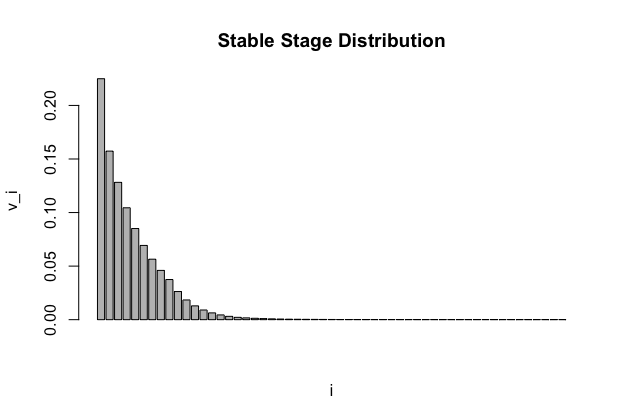
\includegraphics[scale=0.45]{figure_1a.png}
        \end{figure}
        \FloatBarrier
        The vector of reproductive values $w$ is the scaled eigenvector of $A^T$ corresponding to the largest eigenvector.  The scaling constant is $\dfrac{1}{\norm{v*w}_1}$ where $*$ represents component-wise multiplication.  We find
        \begin{align*}
            w \approx \qty[\begin{array}{c}0.2469775 \\ 0.3459336 \\ 1.4807593 \\ 28.6109872 \\ 140.4760701 \\ 125.3097224 \\ 145.1410949\end{array}].
        \end{align*}
        \begin{figure}[ht!]
            \centering
            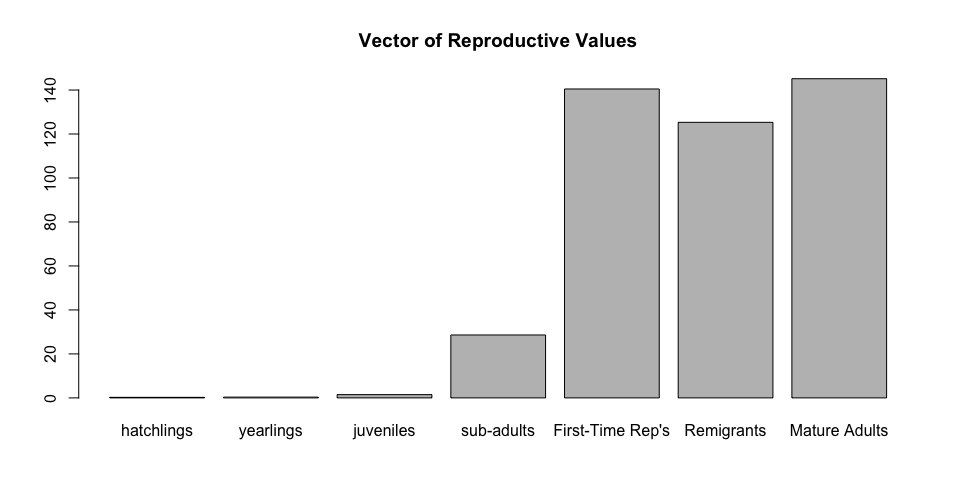
\includegraphics[scale=0.45]{figure_1b.png}
        \end{figure}
        \FloatBarrier
        The stable-stage distribution shows us what we should expect in the long term if $A$ stays constant over time.  That is, that $\sim67\%$ of individuals in the population should be yearlings, $\sim20.7\%$ should be hatchlings, $\sim11.5\%$ should be juveniles, and the rest $<1\%$ are sub-adults, first-time reproducers, re-migrants, and mature adults.  Na\"{i}vely, this might lead us to focus conservation efforts on the hatchlings and yearlings to preserve the distribution.  However, the vector of reproductive values tells us the relative value of each of these stages in terms of what they contribute to future generations.  The mature adults, remigrants, and first-time reproducers have the highest reproductive value, and thus are the most important to reproduction.  Conservation efforts, then, should be focused on preserving what few adults are in the population.  Even though many hatchlings are lost, they have little to no reproductive value anyway.  This is intuitive since based on the matrix $A$, it is highly unlikely that an individual makes it to adulthood.  If the individual makes it to adulthood, however, it is extremely valuable in terms of how many new individuals it can produce.
    \item
        Using $N_0 = \qty[\begin{array}{ccccccc} 10,000 & 0 & 0 & 0 & 0 & 0 & 0\end{array}]^T$, and $\lambda,v,w$ found above, we use the approximation
        \begin{align*}
            N_t \approx 10^4w_1\lambda^{t}v
        \end{align*}
        where $w_1=0.2469775$ is the reproductive number of the hatchlings.  Here are the plots for $t=20$ and $t=100$:
        \begin{figure}[ht!]
            \centering
            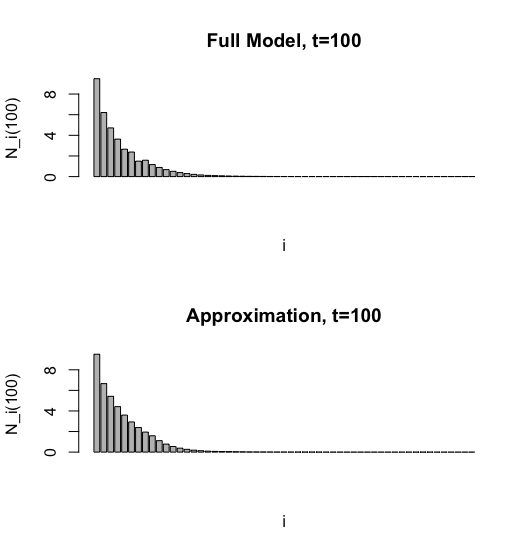
\includegraphics[scale=0.4]{figure_1c.png}
        \end{figure}
        \begin{figure}[ht!]
            \centering
            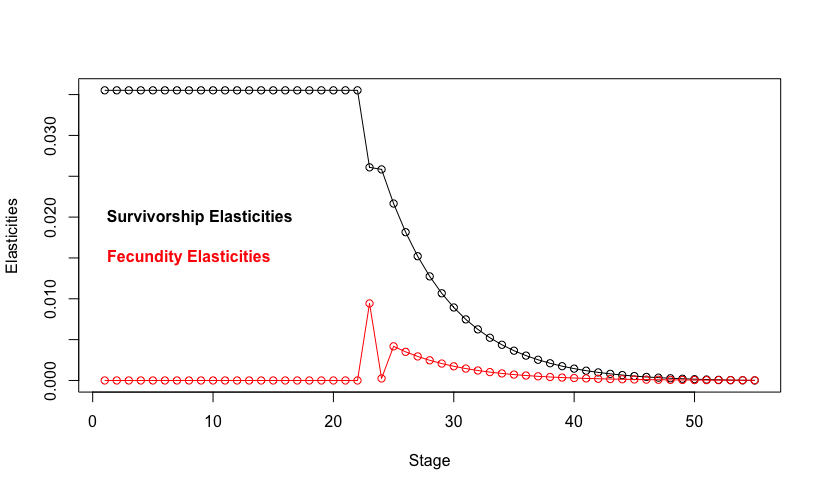
\includegraphics[scale=0.4]{figure_1d.png}
        \end{figure}
        \FloatBarrier
        For $t = 20$, there is an error of about $37$ in the approximation of the yearlings, about $20$ in the approximation of the hatchlings, and about $1$ in the approximation of the juveniles.  All other errors are $\order{0.1}$.  For $t = 100$, all errors are $\order{0.1}$ (the largest error is in the approximation of the hatchlings: about $0.34$).
    \item
        Sensitivities of $\lambda$ to changes in $A$ (notated $S$) are given by the outer product of $w$ with $v$, that is
        \begin{align*}
            S = \qty(\begin{array}{c} w_1 \\ w_2 \\ w_3 \\ w_4 \\ w_5 \\ w_6 \\ w_7 \end{array})\qty(\begin{array}{ccccccc} v_1 & v_2 & v_3 & v_4 & v_5 & v_6 & v_7 \end{array}) = \qty(\begin{array}{ccccccc}
                w_1v_1 & w_1v_2 & w_1v_3 & w_1v_4 & w_1v_5 & w_1v_6 & w_1v_7 \\
                w_2v_1 & w_2v_2 & w_2v_3 & w_2v_4 & w_2v_5 & w_2v_6 & w_2v_7 \\
                w_3v_1 & w_3v_2 & w_3v_3 & w_3v_4 & w_3v_5 & w_3v_6 & w_3v_7 \\
                w_4v_1 & w_4v_2 & w_4v_3 & w_4v_4 & w_4v_5 & w_4v_6 & w_4v_7 \\
                w_5v_1 & w_5v_2 & w_5v_3 & w_5v_4 & w_5v_5 & w_5v_6 & w_5v_7 \\
                w_6v_1 & w_6v_2 & w_6v_3 & w_6v_4 & w_6v_5 & w_6v_6 & w_6v_7 \\
                w_7v_1 & w_7v_2 & w_7v_3 & w_7v_4 & w_7v_5 & w_7v_6 & w_7v_7 \\
            \end{array}).
        \end{align*}
        The elasticities of $\lambda$ to changes in $A$ (notated $E$) are given by $S*A*\frac{1}{\lambda}$, that is
        \begin{align*}
            E = \frac{1}{\lambda}\qty(\begin{array}{ccccccc}
                a_{11}w_1v_1 & a_{12}w_1v_2 & a_{13}w_1v_3 & a_{14}w_1v_4 & a_{15}w_1v_5 & a_{16}w_1v_6 & a_{17}w_1v_7 \\
                a_{21}w_2v_1 & a_{22}w_2v_2 & a_{23}w_2v_3 & a_{24}w_2v_4 & a_{25}w_2v_5 & a_{26}w_2v_6 & a_{27}w_2v_7 \\
                a_{31}w_3v_1 & a_{32}w_3v_2 & a_{33}w_3v_3 & a_{34}w_3v_4 & a_{35}w_3v_5 & a_{36}w_3v_6 & a_{37}w_3v_7 \\
                a_{41}w_4v_1 & a_{42}w_4v_2 & a_{43}w_4v_3 & a_{44}w_4v_4 & a_{45}w_4v_5 & a_{46}w_4v_6 & a_{47}w_4v_7 \\
                a_{51}w_5v_1 & a_{52}w_5v_2 & a_{53}w_5v_3 & a_{54}w_5v_4 & a_{55}w_5v_5 & a_{56}w_5v_6 & a_{57}w_5v_7 \\
                a_{61}w_6v_1 & a_{62}w_6v_2 & a_{63}w_6v_3 & a_{64}w_6v_4 & a_{65}w_6v_5 & a_{66}w_6v_6 & a_{67}w_6v_7 \\
                a_{71}w_7v_1 & a_{72}w_7v_2 & a_{73}w_7v_3 & a_{74}w_7v_4 & a_{75}w_7v_5 & a_{76}w_7v_6 & a_{77}w_7v_7 \\
            \end{array}).
        \end{align*}
        The elasticities associated with fecundity are given by the elements in the first row, which correspond to how many births do individuals in any given stage give.  The elasticities associated with survivorship are given by the sum of the entries on the diagonals and the sub-diagonals since surviving individuals either stay in their class or move on to the next class.  Here is the result:
        \begin{figure}[ht!]
            \centering
            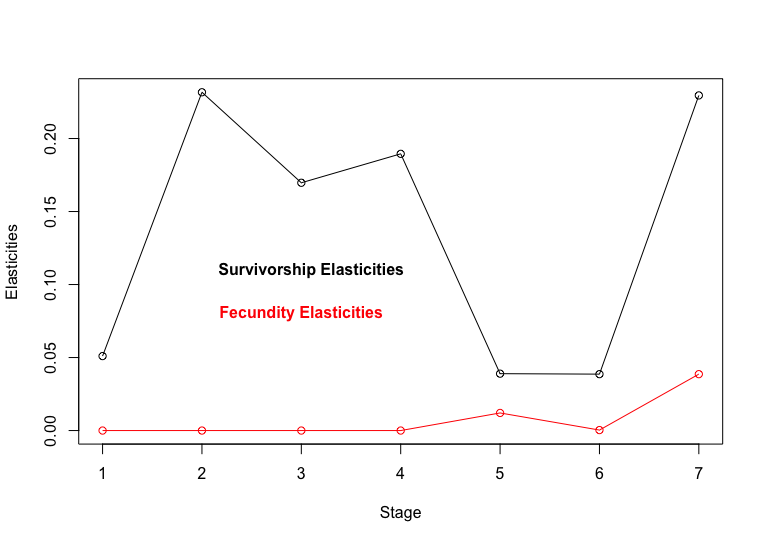
\includegraphics[scale=0.45]{figure_1e.png}
        \end{figure}
        \FloatBarrier
        This shows that $\lambda$ is the most sensitive to survivorship and fecundity of the subclass of mature adults, which is consistent with our analysis of the vector of reproductive values $w$.  In Fig.~3 in Crouse et al.~1987, she separates the elasticities of survival while staying in the same stage, labeled $P_i$, with the elasticities of survival with growth, labeled $G_i$.  My figure above maches perfectly with Crouse's.  My survivorship elasticities are the component-wise sum of Crouse's $P_i$ and $G_i$, as shown in her figure below.
        \begin{figure}[ht!]
            \centering
            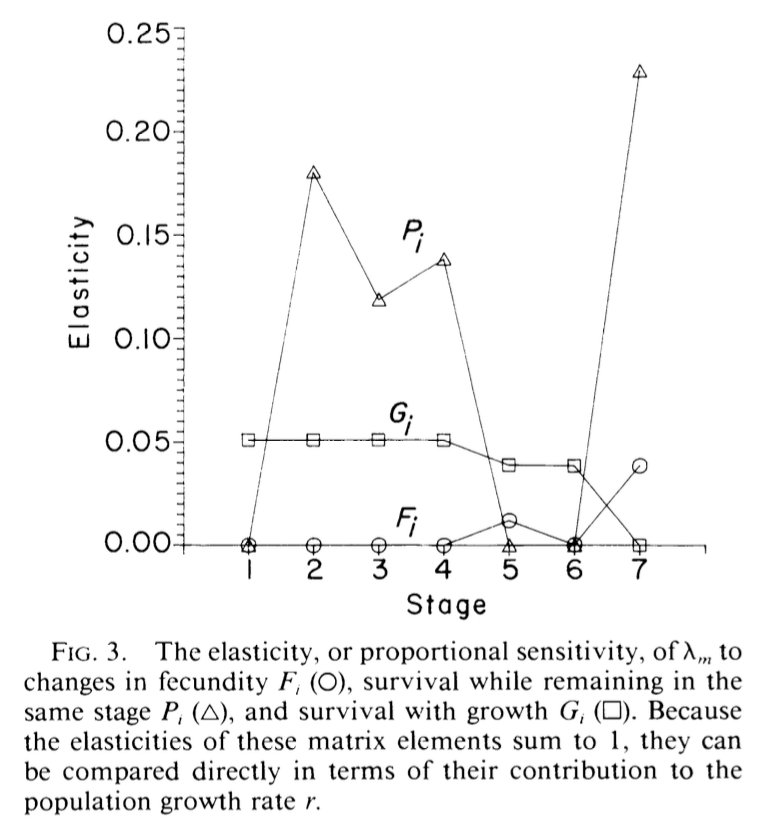
\includegraphics[scale=0.6]{Crouse_et_al_fig_3.png}
        \end{figure}
\end{enumerate}














\end{document}
